
Análise de Insertion Sort: A análise começa com uma descrição detalhada dos custos associados a cada linha do pseudo-código de Insertion Sort. Ela também considera o número de vezes que cada linha é executada, especialmente focando no teste do laço while\cite{cormen2002}.

A análise pode eventualmente ser simplificada, passando de uma fórmula complexa com múltiplos termos para uma notação mais gerenciável e intuitiva, como a notação O big (O), que é mais fácil de usar para comparar a eficiência de diferentes algoritmos.

\begin{figure}[htbp]
    \centering
    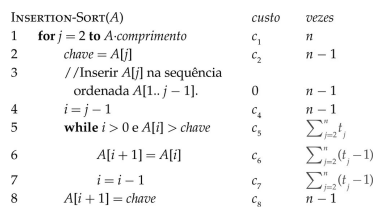
\includegraphics[width = 10cm]{Imagens/Insertion Sort/custosINSERT.png}
    \caption{Tabela sobre o custo do Insertion Sort}
    \label{grafico_insert}
\end{figure}

\begin{figure}[h!]
    \centering
    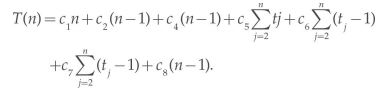
\includegraphics[width = 10cm]{Imagens/Insertion Sort/formula.png}
    \caption{Fórmula para calcular T(n) Insertion Sort.}
    \label{grafico_insert}
\end{figure}



MELHOR CASO: O melhor caso ocorre quando o arranjo já está ordenado. Neste cenário, o algoritmo percorre o arranjo uma única vez, tornando sua complexidade de tempo O(n) conforme equação \eqref{eq:funcao_linear}. 

\begin{equation}
T(n) = C_1n + C_2(n-1) + C_3(n-1) + C_4(n-1) + C_7(n-1)
\end{equation}

Aplicando a distributiva, temos:

\begin{align}
T(n) &= C_1n + (C_2n - C_2) + (C_3n - C_3) + (C_4n - C_4) + (C_7n - C_7) \\
     &= (C_1 + C_2 + C_3 + C_4 + C_7)n - (C_2 + C_3 + C_4 + C_7)
\end{align}

Assim, o resultado é uma função linear:

\begin{equation}
T(n) = An - B \quad \text{(Função linear)}
\label{eq:funcao_linear}
\end{equation}

PIOR CASO: O pior caso acontece quando o arranjo está ordenado em ordem decrescente. Isso força o algoritmo a fazer o máximo de comparações e movimentações, resultando em uma complexidade de tempo O($ n^2 $) conforme equação \eqref{eq:funcao_quadratica}.

\begin{equation}
T(n) = C_1n + C_2(n-1) + C_3(n-1) + C_4\left(\sum_{j=2}^{n} T_j \right) + C_5\left(\sum_{j=2}^{n} (T_j - 1) \right) + C_6\left(\sum_{j=2}^{n} (T_j - 1) \right) + C_7(n - 1)
\end{equation}

que resulta em

\begin{equation}
T(n) = An^2 + Bn + C \quad \text{(Função quadrática)}
\label{eq:funcao_quadratica}
\end{equation}


CASO MÉDIO: Este é o cenário mais representativo para a maioria das aplicações práticas. No caso médio, a complexidade de tempo também é O($ n^2 $), mas o número de comparações e movimentações é, em média, menor do que no pior caso.
Cálculo médio caso: \begin{equation}
T(n) = C_1n + C_2(n-1) + C_3(n-1) + C_4\left(\sum_{j=2}^{n} T_j\right) + C_5\left(\sum_{j=2}^{n}(T_j - 1)\right) + C_6\left(\sum_{j=2}^{n}(T_j - 1)\right) + C_7(n - 1)
\end{equation}
Que resulta em T(n)=A$ n^2 $ + Bn + C(Função quadrática).

